\documentclass[tikz,border=8pt]{standalone}
\usepackage{ctex}
\usepackage{amsmath,amssymb}
\usetikzlibrary{arrows.meta,calc,angles,quotes,positioning,decorations.pathreplacing}
\definecolor{ink}{RGB}{31,43,57}
\definecolor{blue}{RGB}{35,91,166}
\definecolor{orange}{RGB}{224,111,20}
\definecolor{green}{RGB}{35,139,92}
\definecolor{red}{RGB}{190,52,52}
\tikzset{
 line cap=round,line join=round,
 body/.style={draw=ink,very thick},
 vec/.style={-{Latex[length=2.5mm]},draw=blue,very thick},
 force/.style={-{Latex[length=2.5mm]},draw=red,very thick},
 guide/.style={draw=ink!45,dashed},
 dim/.style={{Latex[length=2mm]}-{Latex[length=2mm]},draw=ink!70}
}
\begin{document}

% question-01
\begin{tikzpicture}[scale=.95]
 \fill[ink!7] (-1.05,-.55) rectangle (1.05,.2);
 \draw[body] (-1.05,.2)--(1.05,.2);
 \draw[body] (-4.2,-.367)--(4.2,1.145);
 \fill[orange] (-4.2,-.367) circle(3.5pt) node[below left] {$A$};
 \fill[orange] (4.2,1.145) circle(3.5pt) node[above right] {$B$};
 \draw[dim] (-1.05,-1.0)--(1.05,-1.0) node[midway,below] {$l$};
 \draw[dim] (-4.2,-1.65)--(4.2,-1.65) node[midway,below] {$L$};
 \draw[guide] (-4.8,.2)--(4.8,.2);
 \coordinate (Q1X) at (4.2,.2);
 \coordinate (Q1O) at (-1.05,.2);
 \coordinate (Q1B) at (4.2,1.145);
 \draw pic[draw=blue,very thick,angle radius=16mm,"$\varphi_0$"] {angle=Q1X--Q1O--Q1B};
 \node at (0,1.55) {均匀杆在相距 $l$ 的两个支承端点间交替转动};
\end{tikzpicture}

% solution-01
\begin{tikzpicture}[scale=.9]
 \draw[body] (-4,0)--(4,0);
 \fill[ink!15] (-1,-.6) rectangle (1,-.12);
 \fill[orange] (-1,0) circle(3pt) node[below left] {$P$};
 \fill[orange] (1,0) circle(3pt) node[below right] {$Q$};
 \fill[ink] (0,0) circle(3pt) node[below] {$C$};
 \draw[force] (1,.12)--(1,1.5) node[right] {$J$};
 \draw[vec] (0,.12)--(0,1.1) node[left] {$v_C^+$};
 \draw[vec] (2,0)--(2,1.35) node[right] {$v_Q^+=2ea\Omega$};
 \node[align=center] at (0,2.3) {$e>0$ 时碰后 $Q$ 离开支承，不能立即作为固定支点};
 \node[align=center,draw=ink!30,fill=white] at (0,-1.7)
 {$\eta=3l^2/L^2$，\quad $J=2ma(1+e)\Omega/(1+\eta)$\\
 $\Delta K/K^-=4\eta(1-e^2)/(1+\eta)^2$};
\end{tikzpicture}

% question-02
\begin{tikzpicture}[scale=.82]
 \begin{scope}[xshift=-5cm,yshift=2cm]
  \draw[body] (-2.5,1)--(2.5,1) node[right] {$I$};
  \draw[body] (-2,-1)--(2,-1) node[right] {$I'$};
  \fill[orange] (0,-1) circle(3pt);
  \draw[dim] (-2.7,-1)--(-2.7,1) node[midway,left] {$d$};
  \node at (0,-1.65) {可转动载流铁棒};
 \end{scope}
 \begin{scope}[xshift=3.5cm,yshift=2cm]
  \draw[body] (-2.7,0)--(0,0);
  \draw[body] (0,0)--(2.8,1.2) (0,0)--(2.8,-1.2);
  \draw[guide] (0,0) ellipse(.38 and 1.18);
  \draw[guide] (2.8,0) ellipse(.52 and 1.2);
  \draw[vec] (-1.8,0)--(-.65,0) node[midway,above] {$I$};
  \coordinate (Q2L) at (2.8,-1.2);
  \coordinate (Q2O) at (0,0);
  \coordinate (Q2U) at (2.8,1.2);
  \draw pic[draw=orange,very thick,angle radius=9mm,"$\Omega$"] {angle=Q2L--Q2O--Q2U};
  \node at (.6,-1.75) {圆锥面向外流};
 \end{scope}
 \begin{scope}[xshift=-4.5cm,yshift=-2.2cm]
  \fill[blue!6] (-2.6,-.12) rectangle (2.6,.12);
  \draw[body] (-2.6,0)--(2.6,0);
  \draw[vec] (0,1.75)--(0,.25) node[midway,right] {$I$};
  \foreach \a in {20,50,80,110,140,170,200,230,260,290,320,350}{\draw[orange,thick,-{Latex[length=1.8mm]}] (0,0)--++(\a:1.55);}
  \node at (0,-1.85) {无限导体平面径向电流};
 \end{scope}
 \begin{scope}[xshift=3.8cm,yshift=-2.2cm]
  \fill[blue!5] (0,0) circle(1.55); \draw[body] (0,0) circle(1.55);
  \draw[body] (0,2.05)--(0,1.55) (0,-1.55)--(0,-2.55);
  \draw[vec] (0,2.0)--(0,1.7) node[right] {$I$};
  \foreach \a in {60,90,120}{\draw[orange,thick,-{Latex[length=1.7mm]}] (\a:1.55) arc[start angle=\a,end angle=-\a,radius=1.55];}
  \node at (0,-3.0) {球壳表面电流};
 \end{scope}
\end{tikzpicture}

% solution-02
\begin{tikzpicture}[scale=.9]
 \begin{scope}[xshift=-4.5cm]
  \draw[-{Latex[length=2mm]},body] (0,-2.4)--(0,2.5) node[left] {$B_\varphi$};
  \draw[-{Latex[length=2mm]},body] (-.2,0)--(3.5,0) node[below] {$r$};
  \draw[blue,very thick,domain=.35:3.2,samples=70] plot(\x,{1.25/\x});
  \node[blue,align=left] at (2.1,1.8) {$\displaystyle B=\frac{\mu_0I}{2\pi r}$\\长直导线};
  \draw[orange,very thick] (.3,-1.2)--(3.2,-1.2);
  \node[orange] at (1.8,-1.65) {$B_\parallel=\mu_0J/2$（孤立均匀电流面）};
 \end{scope}
 \begin{scope}[xshift=4.2cm]
  \draw[body] (-3,0)--(3,0);
  \draw[vec] (-1.2,1.7)--(-1.2,.3) node[midway,left] {$B_1$};
  \draw[vec] (1.2,1.7)--(1.2,.3) node[midway,right] {$B_2$};
  \draw[force] (0,0)--++(0,-1.4) node[right] {$p$};
  \node[draw=ink!35,rounded corners,fill=white,align=center] at (0,-2.4)
  {$\displaystyle J=\frac{B_1-B_2}{\mu_0}$，\quad
   $\displaystyle p=\frac{B_1^2-B_2^2}{2\mu_0}$};
  \node[align=center] at (0,2.55) {磁场边界条件与磁压};
 \end{scope}
\end{tikzpicture}

% question-03
\begin{tikzpicture}[scale=1.1]
 \draw[guide] (-3.5,0)--(3.7,0);
 \draw[body] (-1.5,0) circle(1.5) (1.5,0) circle(1.5);
 \fill[orange] (-.2925,0) circle(3pt);
 \draw[guide] (-.2925,0)--(-.2925,.85);
 \draw[dim] (-.2925,.7)--(0,.7);
 \node[align=center] at (-.8,2.25) {小虫在左泡内\\$a=0.195R$};
 \node[below] at (-.2925,-.08) {$S$};
 \node[below right] at (0,0) {相切点};
 \draw[dim] (-1.5,-.7)--(0,-.7) node[midway,below] {$R$};
 \node at (0,-2.1) {泡内为空气，周围液体折射率为 $n$};
\end{tikzpicture}

% solution-03
\begin{tikzpicture}[x=2.4cm,y=1cm]
 \draw[-{Latex[length=2mm]},ink!55] (-1.0,0)--(2.6,0) node[right] {$x/R$};
 \draw[body] (0,-.8)--(0,.9) (2,-.8)--(2,.9);
 \fill[orange] (-.195,0) circle(2.5pt) node[above left] {$S:-0.195$};
 \fill[blue] (-.172584,0) circle(2.5pt);
 \draw[guide] (-.172584,0)--(-.172584,-1.0);
 \node[below,blue] at (-.172584,-1.0) {$u/R=-0.172584$};
 \fill[red] (.319672,0) circle(2.5pt) node[above right] {$x_r/R=0.319672$};
 \node[above] at (0,1.1) {相切的两个界面};
 \node[above] at (2,1.1) {最后折射面};
 \draw[dim] (.319672,-.5)--(2,-.5) node[midway,below] {$v/R=-1.680328$};
 \node[align=center] at (.85,-2.1) {$\Phi_c=-2(n-1)/R$，\quad $p=2R-u$\\$n=1.3330398$ 时两支虚像坐标相同};
\end{tikzpicture}

% question-04
\begin{tikzpicture}[scale=.9]
 \fill[ink] (0,2.7) circle(3pt);
 \draw[body] (0,2.7)--(-.65,.55)--(.45,-1.65);
 \shade[ball color=orange!45] (-.65,.55) circle(.23) node[left=5pt] {$A,m$};
 \shade[ball color=orange!45] (.45,-1.65) circle(.23) node[below right=3pt] {$B,m$};
 \node[fill=white,inner sep=1pt] at (-.55,1.7) {$l_1$};
 \node[fill=white,inner sep=1pt] at (.02,-.55) {$l_2$};
 \draw[guide] (0,2.7)--(0,-2.1);
 \node at (0,-2.75) {两级等质量复摆，绳长随温度改变};
\end{tikzpicture}

% solution-04
\begin{tikzpicture}[scale=.9]
 \begin{scope}[xshift=-3cm]
  \draw[body] (0,2)--(-.45,.35)--(-.9,-1.3);
  \fill[orange] (-.45,.35) circle(4pt); \fill[orange] (-.9,-1.3) circle(4pt);
  \draw[vec] (.1,.3)--++(-.7,0) node[left] {同相};
  \node at (0,-2) {$\omega_-^2=(2-\sqrt2)g/l_0$};
 \end{scope}
 \begin{scope}[xshift=3cm]
  \draw[body] (0,2)--(.45,.35)--(-.25,-1.35);
  \fill[orange] (.45,.35) circle(4pt); \fill[orange] (-.25,-1.35) circle(4pt);
  \draw[vec] (.25,.25)--++(.75,0) node[right] {反相};
  \draw[vec] (-.1,-1.35)--++(-.75,0);
  \node at (0,-2) {$\omega_+^2=(2+\sqrt2)g/l_0$};
 \end{scope}
 \node[align=center] at (0,3) {$\alpha_1+\alpha_2=0$ 时两支频率的一阶温漂同时消失};
\end{tikzpicture}

% question-05
\begin{tikzpicture}[scale=.87]
 \fill[orange] (0,0) circle(.35) node[below=6pt] {太阳};
 \draw[body] (0,0) circle(1.55); \draw[body] (0,0) circle(4.0);
 % 转移椭圆以太阳为焦点，近日点在地球轨道、远日点在木星轨道
 \draw[blue,very thick] (-1.225,0) ellipse(2.775 and 2.49);
 \fill[blue] (1.55,0) circle(4pt) node[below] {地球};
 \fill[red] (-4,0) circle(4pt) node[left] {木星};
 \draw[vec] (1.55,0)--++(0,1.1) node[right] {$v_1$};
 \node[blue] at (0,1.9) {Juno 转移椭圆};
 \draw[dim] (0,-4.55)--(4,-4.55) node[midway,below] {$R_J$};
\end{tikzpicture}

% solution-05
\begin{tikzpicture}[scale=1.2]
 \draw[-{Latex[length=2mm]},body] (-.3,0)--(4.4,0) node[right] {$v_x$};
 \draw[-{Latex[length=2mm]},body] (0,-.3)--(0,1.5) node[left] {$v_y$};
 \draw[vec] (0,0)--(3,0) node[midway,below] {$\boldsymbol v_E$};
 \draw[vec] (0,0)--(3.426,.776) node[midway,above] {$\boldsymbol v_{\rm in}$};
 \draw[vec] (3,0)--(3.426,.776) node[above right] {$\boldsymbol u_{\rm in}$};
 \draw[orange,very thick,-{Latex[length=2mm]}] (3,0)--(3.885,0) node[midway,below=8pt] {$\boldsymbol u_{\rm out}$};
 \draw[guide] (3.885,0) arc[start angle=0,end angle=61.2,radius=.885];
 \node[align=center] at (2,2.2) {飞掠前后地心相对速度箭头等长\\$|\boldsymbol u_{\rm in}|=|\boldsymbol u_{\rm out}|=8.821\,\mathrm{km/s}$};
\end{tikzpicture}

% question-06
\begin{tikzpicture}[scale=.9]
 \begin{scope}[xshift=-3.8cm]
  \draw[-{Latex[length=2.3mm]},body] (0,0)--(4,0) node[below] {$x$};
  \draw[-{Latex[length=2.3mm]},body] (0,0)--(0,3) node[left] {$z$};
  \draw[blue,very thick,domain=0:3.4,samples=80] plot(\x,{1.65*\x-.48*\x*\x});
  \draw[vec] (0,0)--(1.0,1.65) node[above] {$v_0,\theta_0$};
  \node at (1.8,-.7) {抛体事件轨迹};
 \end{scope}
 \begin{scope}[xshift=4cm]
  \draw[body] (-2,-1.3) rectangle (2,1.3);
  \fill[orange] (1.35,0) circle(3pt) node[above] {$A$};
  \fill[blue] (-1.35,0) circle(3pt) node[above] {$B$};
  \draw[vec] (1.25,0)--(-1.15,0) node[midway,above] {激光};
  \draw[dim] (-1.35,-.55)--(1.35,-.55) node[midway,below] {$d$};
  \draw[force] (0,-1.5)--++(0,-1.0) node[right] {$\boldsymbol g$};
  \node at (0,2.1) {横向分离的加速飞船};
 \end{scope}
\end{tikzpicture}

% solution-06
\begin{tikzpicture}[scale=.95]
 \begin{scope}[xshift=-4.2cm]
  \draw[-{Latex[length=2mm]},body] (0,0)--(3.2,0) node[right] {$ct$};
  \draw[-{Latex[length=2mm]},body] (0,0)--(0,2.5) node[left] {$z$};
  \draw[blue,very thick,domain=0:3,samples=50] plot(\x,{1.4*\x-.47*\x*\x});
  \fill[orange] (1.49,1.04) circle(3pt) node[above] {顶点};
  \node[align=center] at (1.5,-1) {事件曲线的 $ct-z$ 投影\\$R_{E,\rm top}=(c^2+v_x^2)/g$};
 \end{scope}
 \begin{scope}[xshift=3.8cm]
  \draw[body] (-2,-.8) rectangle (2,1.7);
  \fill[orange] (1.3,0) circle(3pt) node[above] {$A$};
  \fill[blue] (-1.3,0) circle(3pt) node[above] {$B$};
  \draw[vec] (1.2,-.1)--(-1.2,-.65) node[midway,above] {瞄准};
  \draw[force] (2.3,1)--(2.3,-.5) node[right] {$g$};
  \node[align=center] at (0,-1.6) {相同 Rindler 高度：$f_B=f_A$\\$\tan\chi=gd/(2c^2)$};
 \end{scope}
\end{tikzpicture}

% question-07
\begin{tikzpicture}[scale=.95]
 \draw[body] (-5,-.7)--(5,-.7);
 \foreach \x/\lab in {-2.8/A,-.2/B,2.4/C}{\shade[ball color=orange!45] (\x,0) circle(.34) node[above=6pt] {$\lab$};}
 \draw[vec] (-4.5,0)--(-3.35,0) node[midway,above] {$v_0$};
 \draw[guide] (-2.45,0)--(-.55,0);
 \node at (0,-1.45) {三个等质量小球的一维或非共线弹性碰撞};
\end{tikzpicture}

% solution-07
\begin{tikzpicture}[scale=.86]
 \begin{scope}[xshift=-4cm,x=2.45cm,y=2.45cm]
  \draw[-{Latex[length=2mm]},body] (-.48,0)--(1.25,0) node[below] {$v_2/v_0$};
  \draw[-{Latex[length=2mm]},body] (0,-.48)--(0,1.25) node[left] {$v_3/v_0$};
  \draw[blue,very thick,domain=0:360,samples=160,smooth]
   plot ({1/3+1/3*cos(\x)+1/sqrt(3)*sin(\x)},
         {1/3+1/3*cos(\x)-1/sqrt(3)*sin(\x)});
  \draw[guide,dashed] (-.35,-.35)--(1.12,1.12) node[above right] {$y=x$};
  \draw[guide,dashed] (-.05,1.1)--(.72,-.44) node[below right] {$2x+y=1$};
  \draw[red,very thick,domain=-60:0,samples=50,smooth]
   plot ({1/3+1/3*cos(\x)+1/sqrt(3)*sin(\x)},
         {1/3+1/3*cos(\x)-1/sqrt(3)*sin(\x)});
  \fill[red] (0,1) circle(1.4pt) node[left=3pt] {$(0,1)$};
  \fill[red] (2/3,2/3) circle(1.4pt) node[above right] {$(2/3,2/3)$};
  \node[red,align=center] at (.28,.75) {允许弧};
  \node[align=center] at (.38,-1.0) {$x^2+y^2+xy-x-y=0$};
 \end{scope}
 \begin{scope}[xshift=4cm,x=2.45cm,y=2.45cm]
  \draw[-{Latex[length=2mm]},body] (-.5,0)--(1.3,0) node[below] {$v_{2x}/v_0$};
  \draw[-{Latex[length=2mm]},body] (0,-.85)--(0,.9) node[left] {$v_{2y}/v_0$};
  \fill[blue!8] (1/3,0) circle(2/3); \draw[blue,very thick] (1/3,0) circle(2/3);
  \fill[orange] (1/3,0) circle(3pt) node[below right] {$(1/3,0)$};
  \node at (.4,-1.1) {$\displaystyle (x-1/3)^2+y^2\le(2/3)^2$};
 \end{scope}
\end{tikzpicture}

% question-08
\begin{tikzpicture}[scale=.95]
 \draw[body] (0,0) circle(2.15);
 \foreach \a/\lab in {90/v_1,210/v_2,330/v_3}{
  \coordinate (P) at (\a:2.15);
  \draw[guide] (0,0)--(P);
  \draw[body] (P)--++({\a-90}:2.2);
  \draw[vec] ($(P)+({\a-90}:1.0)$)--++({\a-90}:.9) node[above] {$\lab$};
 }
 \fill[ink] (0,0) circle(3pt) node[below right] {$C$};
 \node at (0,-3.7) {三条切线的切点互差 $120^\circ$};
\end{tikzpicture}

% solution-08
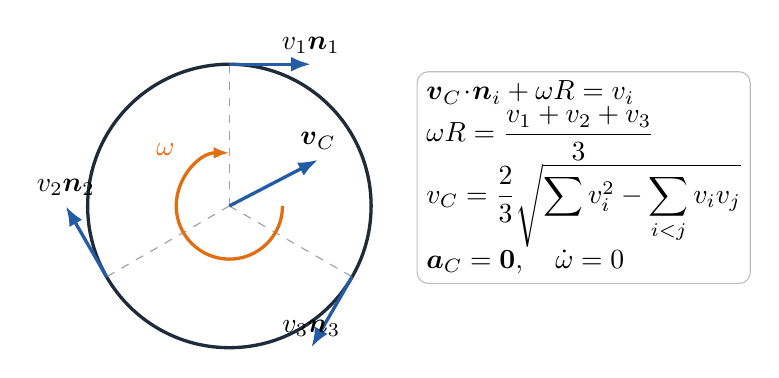
\begin{tikzpicture}[scale=.9]
 \draw[body] (0,0) circle(2.0);
 \foreach \a/\i in {90/1,210/2,330/3}{
  \coordinate (P\i) at (\a:2);
  \draw[guide] (0,0)--(P\i);
  \draw[vec] (P\i)--++({\a-90}:1.15) node[above] {$v_\i\boldsymbol n_\i$};
 }
 \draw[vec] (0,0)--(1.25,.65) node[above] {$\boldsymbol v_C$};
 \draw[orange,very thick,-{Latex[length=2mm]}] (.75,0) arc[start angle=0,end angle=-270,radius=.75];
 \node[orange] at (-.9,.8) {$\omega$};
 \node[align=left,draw=ink!30,rounded corners,fill=white] at (5,.4)
 {$\boldsymbol v_C\!\cdot\!\boldsymbol n_i+\omega R=v_i$\\
  $\displaystyle \omega R=\frac{v_1+v_2+v_3}{3}$\\
  $\displaystyle v_C=\frac23\sqrt{\sum v_i^2-\sum_{i<j}v_iv_j}$\\
  $\boldsymbol a_C=\boldsymbol0,\quad\dot\omega=0$};
\end{tikzpicture}

\end{document}
